\documentclass{standalone}
\usepackage{pgfplots}
\begin{document}
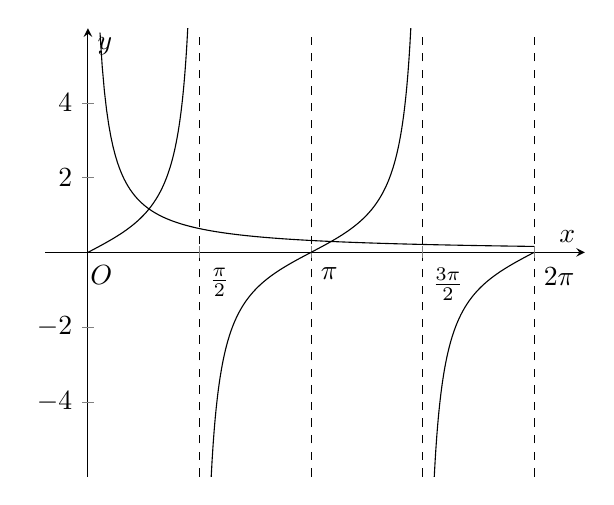
\begin{tikzpicture}
\begin{axis}
[
ymin=-6,ymax=6,
xmin=-0.6,xmax=7,
xtick=\empty,
ytick=\empty,
extra x ticks={1.5708, 3.14159, 4.71239, 6.28319},
extra x tick labels={$\frac{\pi}{2}$, $\pi$, $\frac{3\pi}{2}$, $2\pi$},
extra y ticks={-4, -2, 2, 4},
extra y tick labels={$-4$, $-2$, $2$, $4$},
every extra x tick/.style={
    xticklabel style={anchor=north west},
    grid=major,
    major grid style={very thin,dashed,black}
},
axis lines = center,
xlabel=$x$,ylabel=$y$,
samples=200,
]
\addplot [black, domain=0:1.4508] {tan(deg(x))};
\addplot [black, domain=1.6908:4.59239] {tan(deg(x))};
\addplot [black, domain=4.83239:6.28319] {tan(deg(x))};
\addplot [black, domain=0.17:6.28319] {1/x};
\node at (axis cs:0.19, -0.6) {$O$} ;
\end{axis}
\end{tikzpicture}
\end{document}
